\chapter{Origen}

\section{Origen histórico}

El origen de Scrum se remonta a la década del 80. La revista gerencial "Harvard Business Review" publica un artículo de Takeuchi y Nonaka denominado: "El nuevo nuevo juego para el desarrollo de productos" \cite{Takeuchi-Nonaka-1986}. En el artículo se describe cómo empresas tales como Honda, Canon y Fuji-Xerox producían nuevos productos a nivel mundial utilizando un enfoque diferente al tradicional de entonces. En ese artículo se introdujo el concepto Scrum, con el término tomado del deporte Rugby, para simbolizar este nuevo enfoque basado en equipos integrales para el desarrollo de productos. Hay autores que denominan a estos conceptos originales de Scrum como "Scrum pragmático" \cite{ScrumManager-2014}.

Una década más tarde, Jeff Sutherland y su equipo en Easel Corporation crearon el proceso de Scrum para ser utilizado en los procesos de 
desarrollo de software tomando los conceptos del artículo original de Takeuchi y Nonaka. Luego, en 1995, Jeff Sutherland junto con Ken Schwaber publican un informe sobre Scrum en una conferencia de Programación Orientada a Objetos OOPSLA. El informe fue formalizado con el nombre Proceso de Desarrollo SCRUM \cite{Ken-Schwaber-1995}. Hay autores que denominan a este marco de reglas para desarrollo de software como "Scrum técnico" \cite{ScrumManager-2014}. Desde esa fecha, Schwaber and Sutherland, han producido y publicado varias especificaciones para Scrum que han servido como guías y material de referencia; como por ejemplo: "Agile software development with Scrum" \cite{Ken-Schwaber-2002} y "The Scrum Guide" \cite{Ken-Jeff-2013}.

Luego, en los 90, Scrum paso a ser reconocidamente parte de las llamadas "Metodologías de Desarrollo de Software de peso liviano", junto a Crystal (1992), Feature Driven Development (1997), Desarrollo de Software Adaptativo (1999) y Extreme Programming (1999). Y luego del Manifiesto Ágil \cite{Beck-2001}, promulgado en 2001 y firmado por Ken y Jeff, pasó a ser reconocida como parte del movimiento ágil y su filosofía. Ken Schwaber fue el primer presidente de la Alianza Ágil fundada tras el Manifiesto Ágil.

Desde que surgió se popularizó en en el mundo industrial, principalmente en la industria de software, miles de proyectos en todo el mundo han utilizado Scrum para el desarrollo de productos, tanto en empresas pequeñas (startups) como en multinacionales. Debido a su amplia aplicación surgieron diferentes entidades capacitadoras y certificadoras para difundir Scrum y certificar el conocimiento de quienes rinden los respectivos exámenes necesarios. La Scrum Alliance \cite{Scrum-Alliance-2015} es un ejemplo de este tipo de organizaciónes y es considerada la principal organización certificante. La Scrum Alliance fue fundada en 2002 por Ken Schwabe, Mike Cohn y Esther Derby. En 2006, Jeff Sutherland creó su propia compañía llamada Scrum.inc, sin dejar de ofrecer y enseñar a los cursos de Certified Scrum. A su vez, Ken dejó la Alianza Scrum en 2009 para fundar la Scrum.org para mejorar aún más la calidad y la eficacia de Scrum, principalmente a través de la serie Profesional Scrum ("Professional Scrum series"). Hay otras organizaciones capacitadoras y certificadoras como ScrumStudy que es una empresa (subsidiaria de VMEdu) que se basa en el libro "SBOK Guide" \cite{SBOK-2013}.

\section{Origen causal}

Scrum tuvo un origen causal que suele constituir el análisis crítico previo a su explicación. Scrum emerge del intento de resolver un problema y de la crítica a las consideradas causas del mismo. Scrum vino a surgir como una alternativa al modo en que se desarrollaba software y lo hizo como posible solución a los problemas que presentaba la situación en ese entonces (década del 90) de Desarrollo de Software. Por esa razón es que por lo general cuando se habla de Scrum se hace un análisis crítico previo para plantear un cambio debido a un problema. Por un lado, Scrum plantea un cambio paradigmático o filosófico que consiste en un cambio de perspectiva y de mentalidad (mindset). La otra cuestión fundamental es la metodológica en la cual se propone un cambio del proceso de desarrollo de software o proceso industrial de software. Por este motivo, para comenzar a comprender Scrum, hay que comprender cuál es el problema que viene a intentar resolver y qué es lo que se critica.

\subsection{Problema}

El problema principal por el que Scrum surgió como alternativa consistió en que la mayoría de los proyectos de desarrollo de software no lograban entregarse en tiempo, dentro de los costos y con las funcionalidades comprometidas. Ya en la primera conferencia organizada por la OTAN (en 1968) sobre desarrollo de software se hablaba de la "Crisis del Software" haciendo mención de los problemas recurrentes en que se veía afectado el desarrollo de software y sus resultados. En ese momento se identificaron entre diversos problemas la baja calidad del software que se desarrollaba, el no cumplimiento de las especificaciones y el código prácticamente inmantenible que dificultaba la gestión y la evolución de los proyectos. Una encuesta de cientos de proyectos de desarrollo de software empresarial indicó que cinco de seis proyectos de software se consideraban no satisfactorios \cite{AntiPatterns-1998}, por otro lado sólo 29 de cada 100 proyectos de IT se terminaban exitosamente y el 71 por ciento de los clientes no estaban satisfechos con los resultados (Standish Groups Chaos Report 1994 - 2004). En el año 1994 el Standish Group publicó un estudio conocido como el "CHAOS Report" \cite{CHAOS-Report-1994} donde se mostró las siguientes tasas de fracaso en los proyectos de desarrollo de software en general:

\begin{itemize}

\item \textbf{Proyectos cancelados:} el 31.1 por ciento es cancelado en algún punto durante el desarrollo del mismo.
\item \textbf{Proyectos insuficiente:} el 52.7 por ciento es entregado con sobrecostos, en forma tardía o con menos funcionalidades de las inicialmente acordadas.

%Las conclusiones de la investigación sugieren que el involucramiento del usuario y el empleo de periodos de tiempo más cortos son claves para incrementar las tasas de proyectos exitosos

\end{itemize}

\subsubsection{Causas}

Los problemas detectados en los modelos tradicionales se fundamentan principalmente en lo siguiente: 

\begin{itemize}

\item \textbf{Entorno cambiante:} Entorno altamente cambiante propio de la industria \cite{Martin-Alaimo-2014}.

\item \textbf{Dependencia de Procesos rígidos:} el proceso mismo de desarrollo de software donde el resultado depende de la actividad
cognitiva de las personas más que de las prácticas y controles de empleados \cite{Martin-Alaimo-2014}. Las metodologías de desarrollo de software resultaron muy pesadas y prohibitivas para responder satisfactoriamente a los cambios de negocio.

\end{itemize}

\subsection{Filosofía criticada}

Como se dijo antes, con Scrum se plantea un cambio paradigmático o filosófico que consiste en un cambio de perspectiva y de mentalidad (mindset).

\subsection{Metodología criticada}

La causa de los problemas y fracasos de los proyectos de software en la situación dada, en ese entonces, de Desarrollo fueron atribuidos principalmente a la Metodología Cascada (Waterfall Methodology) \cite{Ken-Schwaber-1995}. Pero hay que tener en cuenta de qué se habla cuando se critica a la metodología cascada. Pues la metodología cascada no es el modelo cascada y en ocaciones se han atribuido, en un sentido erróneo, las causas de los problemas al modelo cascada. Pues no se puede comparar Scrum con el modelo Cascada porque Scrum no es exactamente un modelo y ofrece soluciones a aspectos que el modelo cascada no ofrece. Aunque si, el modelo cascada, es perte de lo que se podría considerar una Metodología Cascada. 

\subsubsection{Modelo en Cascada}

El Modelo en Cascada (Waterfall Methodology) \cite{Ken-Schwaber-1995} es un Modelo Secuencial de Procesos para la ingeniería de software presentado por Winston Royce en 1970, aunque ya se venía desarrollando desde antes. Para algunos críticos, el Modelo en Cascada, se convirtió en el modelo metodológico más utilizado dentro de la industria en un período de tiempo. Pero hay que considerar que el modelo solo abarca al sistema de producción o sistema de desarrollo (ver "Development Process" en la figura \ref{fig:WaterfallMethodology}) de la industria, no al de gestión, y es simplemente un modelo, no una metodología.

En un sentido lato y ortodoxo se puede decir que el Modelo en Cascada refleja un proceso lineal y secuencial de un conjunto de procesos o fases independientes dentro de un proyecto. Las fases son: requerimientos (requerimiento del sistema y requerimientos del software), diseño, codificación, pruebas y operación. Según esto y siempre cuando el proceso de desarrollo de un proyecto conste de solo la secuencia de estas fases sin repetición, la principales críticas como desventajas que se hacen son:

\begin{enumerate}

\item \textbf{Previción:} Al tener una face de requerimientos única al comienzo, el producto final es anticipado de antemano \cite{Scrum-Institute-2015}. Esto requiere de cierta previción y certidumbre inicial que en proyectos complejos y cambiantes es poco factible que suceda.

\item \textbf{Requerimientos no necesarios:} Requerimientos elicitados al comienzo del proyecto y luego implementados nunca serán completamente necesitados por el cliente \cite{Scrum-Institute-2015}. O sea que pueden haber requerimientos irrelevantes o inecesariamente implementados, ya sea porque el cliente dejó de tener la necesidad en el transcurso del proyecto o porque la incertidumbre inicial generó una mala elicitación de los mismos.

\item \textbf{Fases separadas:} Cada fase es estrictamente separada \cite{Scrum-Institute-2015}. Por ejemplo una vez que se encuentra completa la fase de requerimientos se procede a una firma de aprobación o "sign-off" que congela dichos requerimientos, y es recién aquí cuando se puede iniciar la fase de diseño, fase donde se crea un plano de modelo o "blueprint" del mismo para que, luego, los programadores lo codifiquen y se prosiga con las pruebas y finalmente el despliegue en operación. Pues en entornos altamente cambiante, propio de la industria de software, esta forma secuencial estricta hace del proceso de desarrollo un proceso “pesadas” (estanco y burocrático) y prohibitivo para responder satisfactoriamente a los factores cambiantes de negocio \cite{Martin-Alaimo-2014}.
%Solución propuesta por scrum:
%Fine-grained requirements are only defined when they are really needed.
%All activities to design, build and test a certain functionality are kept together in one phase.
%Changes are expected and welcomed by Scrum team.

\end{enumerate}

\subsubsection{Gestión de Proyectos Clásica}

\begin{enumerate}

\item \textbf{Planeación predictiva:} La planeación predictiva fue impulsada por el PMI quien ha adoptado el enfoque predictivo y mecanicista para la gestión de proyectos. Planeación predictiva es cuando el alcance del proyecto, el tiempo y el costo requerido para el proyecto se determina lo antes posible y luego durante la ejecución del proyecto se busca seguir y respetar el plan. El éxito (o rendimiento) del enfoque predictivo ha sido menos del 50 por ciento (en tiempo, en la fecha y con la funcionalidad deseada) y Scrum se presenta como alternativa para mejorar esta tasa \cite{Ken-Schwaber-2011}. El enfoque predictivo es útil para producción de volumen alto y fabricación de bajo coste. Sus beneficios resultan de reducir la imprevisibilidad del espacio del problema a través de la estandarización y la repetición. La planificación perfecta, la formación y la repetibilidad son las claves. Planificar y luego hacer una y otra vez. La productividad se optimiza a través de procesos de flujo de trabajo perfecto e invariable, y se optimiza el uso de los recursos (personas o máquinas). Pero esta metodología no se ajusta a proyectos donde hay más novedad que repetibilidad y donde las tecnologías, capacidades y creatividad de las personas son cambiantes. En estos casos hay alta probabilidad de que la predictividad fracase \cite{Ken-Schwaber-2011}.

\item \textbf{Planeación a largo plazo:}

\item \textbf{Gestión de recursos humanos:} En la planificación tradicional las personas son gestionadas como recursos, hasta cierto punto intercambiables, especializados que siguen planes. Sin embargo la productividad, la calidad y la creatividad es mucho mayor si la gente que hace el trabajo también lo planea \cite{Ken-Schwaber-2011}.

\item \textbf{Gerente de Proyecto:} En el marco de Scrum se considera que el papel del gerente de proyecto es contraproducente en un trabajo complejo y creativo \cite{Ken-Schwaber-2011}. La dirección de un gerente en base a un plan puede limitar la creatividad y la inteligencia del equipo en lugar de insentivarla para resolver mejor los problemas. Si se elimina la figura de gerente de proyecto y se delegan sus actividades de gestión en otros roles, junto con un enfoque de auto-organización, se puede mejorar la productividad y la creatividad.

\end{enumerate}

\subsubsection{Metodología en Cascada}

\begin{figure}[h]
  \centering
  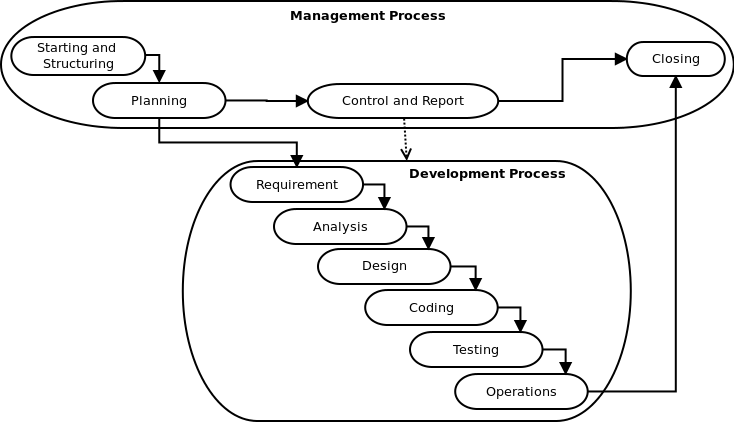
\includegraphics[scale=0.5]{WaterfallMethodology}
  \caption{Metodología Cascada criticada (Diagrama integrador del Modelo Cascada \cite{Winston-Royce-1970}, la Metodología Cascada \cite{Ken-Schwaber-1995} y la Metodología de Gestión de Proyectos \cite{PMBOK-1996})}
  \centering
  \label{fig:WaterfallMethodology} %\ref{fig:WaterfallMethodology}
\end{figure}
